\documentclass[10pt]{extarticle}
\usepackage[paperwidth=9.43in,paperheight=7.07in,margin=0.6in]{geometry}
\usepackage{fontspec}
\setmainfont{Latin Modern Roman}
\directlua{luaotfload.add_fallback("mockfb",{"Apple Symbols:mode=harf;","Apple Braille:mode=harf;","Arial Unicode MS:mode=harf;"})}
\setmonofont{Menlo}[RawFeature={fallback=mockfb}]
\usepackage{fancyvrb}
\usepackage{enumitem}
\usepackage{microtype}
\usepackage{tikz}
\usetikzlibrary{positioning,calc}
\usepackage{booktabs,tabularx}
\usepackage{parskip}
\usepackage{ragged2e}
\RaggedRight
\pagestyle{plain}
\setlist{topsep=0.2em,itemsep=0.25em,parsep=0pt,leftmargin=1em}
\newcolumntype{Y}{>{\RaggedRight\arraybackslash}X}

\newcommand{\you}[2]{{\small[\textbf{you}, #1: \textit{``#2''}]}}
\newcommand{\mock}[1]{\VerbatimInput[fontsize=\fontsize{7}{8.15}\selectfont]{mock/#1.txt}}
\newcommand{\mocksmall}[1]{\VerbatimInput[fontsize=\fontsize{6.4}{7.5}\selectfont]{mock/#1.txt}}

% One screen per page: the mockup at window scale on the left, what it does on the right.
\newcommand{\screen}[4]{%
  \clearpage
  {\large\bfseries #1}\hfill{\small #2}\par\medskip
  \noindent\begin{minipage}[t]{0.69\linewidth}\vspace{0pt}#3\end{minipage}\hfill
  \begin{minipage}[t]{0.28\linewidth}\vspace{0pt}\small #4\end{minipage}\par}

\begin{document}

{\Large\bfseries Locus screens}\\[0.2em]
{\small Version 2, 18 October 2026. Companion to \textit{Locus plan v2}. Every screen with fake data, drawn at the size of your locus window (about 95 by 38 characters), so a page here is close to what you will see beside aulos.}

\medskip
\noindent\begin{minipage}[t]{0.5\linewidth}\vspace{0pt}
\textbf{How to mark these up.} Write on the mockups themselves: cross out what should go, draw where things should move, write what is missing in the margin. A circled \textbf{?} if something is unclear. These marks become design round 1; the ratatui prototype on fixture data follows in your real window \you{18 Oct}{we should for sure have terminal ratatui mockups of the applications with fake data so I can guide how everything should look}.

\medskip
\textbf{Rules every screen follows}
\begin{itemize}
\item A letter in a section's corner focuses it; Enter opens its detail; Esc goes back.
\item \texttt{/} searches, \texttt{?} lists keys, everywhere.
\item Nothing flashes or takes focus. A session that needs you sorts to the top; that is all.
\item Greyscale here; the real screens use your catppuccin colours, one colour per area, matching kairos.
\end{itemize}

\medskip
\textbf{Symbols}\\[0.2em]
{\small\ttfamily ● attended / unread \quad ○ unattended \quad ↻ working \quad ◐ needs you\\ ✓ done \quad ✗ failed \quad ⚠ worth re-checking \quad ◆ find for a project\\ ◇ reading \quad ✦ idea \quad ▲ commits \quad ✎ dossier \quad ✍ ink \quad ? answer}
\end{minipage}\hfill
\begin{minipage}[t]{0.45\linewidth}\vspace{0pt}
\centering
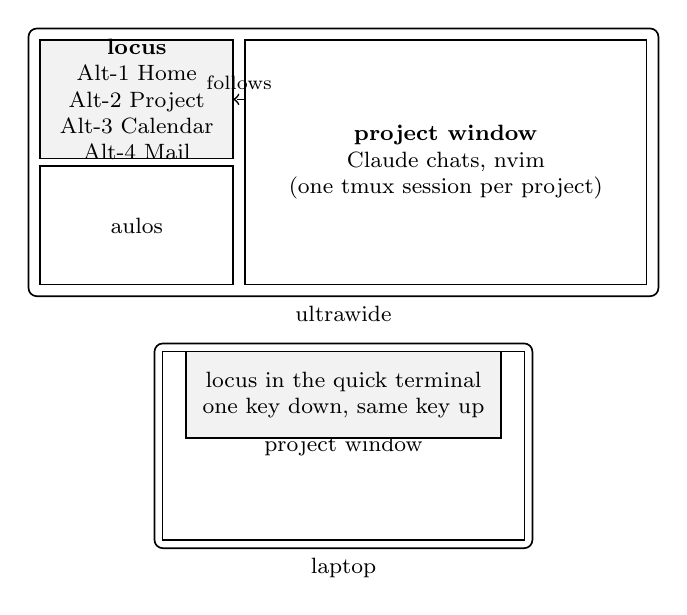
\begin{tikzpicture}[x=1cm,y=1cm,line width=0.6pt,font=\footnotesize]
\draw[rounded corners=3pt] (0,0) rectangle (8,3.4);
\draw[fill=black!5] (0.15,1.75) rectangle (2.6,3.25) node[midway,align=center] {\textbf{locus}\\Alt-1 Home\\Alt-2 Project\\Alt-3 Calendar\\Alt-4 Mail};
\draw (0.15,0.15) rectangle (2.6,1.65) node[midway,align=center] {aulos};
\draw (2.75,0.15) rectangle (7.85,3.25) node[midway,align=center] {\textbf{project window}\\Claude chats, nvim\\(one tmux session per project)};
\draw[->,dashed] (2.75,2.5) -- node[above,font=\scriptsize]{follows} (2.6,2.5);
\node[below] at (4,0) {ultrawide};
\begin{scope}[shift={(1.6,-3.2)}]
\draw[rounded corners=3pt] (0,0) rectangle (4.8,2.6);
\draw (0.1,0.1) rectangle (4.7,2.5) node[midway,align=center] {project window};
\draw[fill=black!5] (0.4,1.4) rectangle (4.4,2.5) node[midway,align=center] {locus in the quick terminal\\one key down, same key up};
\node[below] at (2.4,0) {laptop};
\end{scope}
\end{tikzpicture}
\end{minipage}

% ------------------------------------------------------------------ Home
\screen{Home}{Alt-1}{\mock{home}}{%
\textbf{Next and mail.} One line each, nothing from the calendar repeated \you{18 Oct}{do not want to repeat on home a lot of what the calendar shows}. Alt-3 and Alt-4 jump.

\textbf{Work.} Active hours this week: when you worked, by hour. \texttt{t} colours it by project or kind of work; \texttt{w} opens the area chart over 8 weeks. Backfilled from transcripts since August.

\textbf{Projects.} Every active project, one line each, however many there are. Its sessions, which need you, and unread count. Attended comes from the kairos block or \texttt{m}.

\textbf{Explore and approve.} Finds with their reasoning, graded here or in Explore. Routine approvals beside them, kept separate.

\textbf{System.} Live jobs and the budget; \texttt{l} opens the log of everything done automatically.

\medskip
\textbf{Still open:} is the rhythm grid the right picture? Should approve sit above explore?}

% ------------------------------------------------------------------ Project
\screen{Project}{Alt-2 · follows your project window}{\mock{project}}{%
One screen in every state; while Claude works only the header changes.

\textbf{Where you are.} Three lines, changing slowly: state, where it falls short, the next step.

\textbf{New.} Everything unread, newest first: decisions to re-check, answers, finds, commits, dossier rebuilds, ink. It stays until opened or \texttt{r}. \texttt{n} opens the full timeline. One list for now; it may split by kind later \you{18 Oct}{For now we can put everything new into one place, but that may change later.}

\textbf{Sessions.} Only this project's. Enter jumps your project window there.

\textbf{Chores.} The ones that fit the gap you are in.

\textbf{Ask.} Enter answers here. Tab sends it to the tablet as a learning document.}

% ------------------------------------------------------------------ System
\screen{System}{s from Home, then Enter}{\mock{system}}{%
\textbf{Running} updates live: every job reports its start, steps and end, and elapsed times tick.

\textbf{Recent} keeps failures visible with their cause and what happens next. Nothing fails silently.

\textbf{Usage}: text on the left, thin bars on the right, every row aligned \you{18 Oct}{text should be on one side/ area, and thin bars in another}. The dotted mark is the 15\% cap, or the 60\% line at which background jobs stop for you.

\texttt{t} splits each day's bar by job type. The top-jobs rows are where we look first when tuning.}

% ------------------------------------------------------------------ Explore
\screen{Explore}{e from Home, then Enter}{\mock{explore}}{%
\textbf{Queue}: the scout's finds, at most 7, about one a day. When full, the scout waits.

\textbf{Ideas}: your Jot and Explore ideas, ones you handed to the scout and what came back, parked finds, and every new project idea (the fortnight's best marked).

\textbf{Reading}: what is on the tablet in \texttt{/Reading}, in progress or done.

\medskip
Every proposal carries its reasoning. A reading find stays here until you tick it; only then does it go to the tablet \you{18 Oct}{I do not want to push things to the tablet that I then decline, that is a waste}.

The strike reasons teach the scout, and tell us what to fix.}

% ------------------------------------------------------------------ Approve and log
\screen{Approve and the auto log}{a and l from Home}{\mock{approve}\par\medskip\mock{autolog}}{%
\textbf{Approve} is grouped by kind. \texttt{Y} approves a group at once. The ink group is where marks I cannot place are confirmed.

When you have approved the same kind of thing many times, a ``stop asking?'' item appears. Yes moves that kind to automatic, and the list gets shorter for good.

\textbf{The auto log} is live and one key from Home: every automatic action, with undo where it can be undone \you{18 Oct}{always with a place to see a log of what it has automatically done though}.}

% ------------------------------------------------------------------ Decisions
\screen{Decisions}{d from a Project view}{\mock{decisions}}{%
The list on top, the selected decision explained below from the repository's decision log \you{18 Oct}{decisions should have a view where whichever decsion is selected is explained in more detail from the decision log.}

No keep button: decisions are already made. \texttt{?} asks why it was made, drawing on its log entry, the chats where it was decided and the evidence; the answer lands in Answered. \texttt{o} reopens it in the log, where the working chats see it.

A re-check flag clears once you have seen it, with a note that you looked.}

% ------------------------------------------------------------------ Answered and changes
\screen{Answered and Changes}{a and n from a Project view}{\mock{answered}\par\medskip\mock{changes}}{%
\textbf{Answered} holds every answer for the project, from the ask line or a circled \textbf{?}, linked to the passage. \texttt{f} continues the same thread; \texttt{t} sends it to paper.

\textbf{Changes} is the full timeline behind New, from a date you pick with \texttt{▾}. A detail pane for the selected entry may come later \you{18 Oct}{may want similar detailed view for the one being hovered over, but we will see.}}

% ------------------------------------------------------------------ Search and the work visuals
\screen{Search, and the work section}{/ anywhere}{\mock{search}\par\bigskip
\noindent\begin{minipage}[t]{0.5\linewidth}\vspace{0pt}\small\textbf{Rhythm grid} (default)\par\mocksmall{work_rhythm}\end{minipage}\hfill
\begin{minipage}[t]{0.47\linewidth}\vspace{0pt}\small\textbf{Area chart}, one key away\par\mocksmall{work_area}\end{minipage}}{%
\textbf{Search} covers decisions, answers, Explore, notes, the library, chats and dossiers \you{18 Oct}{being able to quickly search over EVERYTHING in the tui would be really really cool}. From Home it searches everything; from a project, that project; Tab widens.

\medskip
\textbf{The work section.} The rhythm grid shows when you work and, coloured by project, whether each deep block stayed on one project. The area chart shows projects rising and fading over 8 weeks, and is the one that sits best beside the aulos visualiser. Both come from transcripts, commits and kairos logs.}

% ------------------------------------------------------------------ Interview prep
\screen{Interview prep}{p from an opportunity's Project view}{\mock{prep}}{%
Each opportunity gets its own Project view (stage and next date as ``where you are''), plus this plan.

You give the details and the time \you{16 Oct}{I should be able to provide interview details and amount of time I want to spend.} It splits the budget across topics weakest first, from your past prep (the Jump Trading log first) and course material, and the sessions become kairos blocks.

One line per practice session, typed or in ink, keeps the confidence bars honest.}

% ------------------------------------------------------------------ Weekly review
\screen{Weekly review}{w from Home, in its weekend slot}{\mock{review}\par\medskip\mocksmall{review_steps}}{%
Opens in a fixed weekend slot; Home shows ``review ready''. Steps run in order of value, each skippable, and it remembers where you stopped. Skip a week and nothing piles up.

\textbf{1} the week at a glance; \textbf{2} decisions worth re-checking; \textbf{3} what is left in Explore; \textbf{4} locus itself: what it got wrong, unused features, the strike tally; \textbf{5} deep blocks for next week across your two or three projects \you{18 Oct}{probably deep focus blocks for two or even three}.

Automatic actions are not reviewed here; they are in the live log.}

\end{document}
